% -*- latex -*-
%-----------------------------------------------------------------------
%;  Copyright (C) 2007
%;  Associated Universities, Inc. Washington DC, USA.
%;
%;  This program is free software; you can redistribute it and/or
%;  modify it under the terms of the GNU General Public License as
%;  published by the Free Software Foundation; either version 2 of
%;  the License, or (at your option) any later version.
%;
%;  This program is distributed in the hope that it will be useful,
%;  but WITHOUT ANY WARRANTY; without even the implied warranty of
%;  MERCHANTABILITY or FITNESS FOR A PARTICULAR PURPOSE.  See the
%;  GNU General Public License for more details.
%;
%;  You should have received a copy of the GNU General Public
%;  License along with this program; if not, write to the Free
%;  Software Foundation, Inc., 675 Massachusetts Ave, Cambridge,
%;  MA 02139, USA.
%;
%;  Correspondence concerning AIPS should be addressed as follows:
%;          Internet email: aipsmail@nrao.edu.
%;          Postal address: AIPS Project Office
%;                          National Radio Astronomy Observatory
%;                          520 Edgemont Road
%;                          Charlottesville, VA 22903-2475 USA
%-----------------------------------------------------------------------
%Body of final AIPSletter for 31 December 2007

\documentclass[twoside]{article}
\usepackage{graphics}

\newcommand{\AIPRELEASE}{December 31, 2007}
\newcommand{\AIPVOLUME}{Volume XXVII}
\newcommand{\AIPNUMBER}{Number 2}
\newcommand{\RELEASENAME}{{\tt 31DEC07}}
\newcommand{\OLDNAME}{{\tt 31DEC06}}
\newcommand{\NEWNAME}{{\tt 31DEC08}}

%macros and title page format for the \AIPS\ letter.
\input LET98.MAC

\newcommand{\MYSpace}{-11pt}

\normalstyle

\section{General developments in \AIPS}

\subsection{Current and future releases}

We have formal \AIPS\ releases on an annual basis.  While we offer a
full binary installation method for both the frozen and development
versions for MacIntosh OS/X (PPC and Intel chips), Solaris, and Linux
systems, all architectures can do a full installation from the source
files.  The current release is called \RELEASENAME\ and is now
``frozen.''  If you took a development copy of this version at some
earlier date, you should use the ``Midnight Job'' (MNJ) to bring it up
to date.  You need to run a MNJ only once in 2008 to convert your copy
of \RELEASENAME\ into the frozen version.  When patches to 2007 are
announced, you may apply them with the MNJ\@.  This \Aipsletter\ is
intended to advise you of corrections and improvements in this
release.

We have begun a new version, called \NEWNAME, which is now under
development by the \AIPS\ Group.  You may fetch and install a complete
copy of this version at any time.  Having fetched \NEWNAME, you may
update your installation whenever you want by running the MNJ which
uses cvs, rsync, and transaction files to copy and compile the code
selectively based on the code changes and compilations we have done.
We expect users to take their source-only or binary version of
\NEWNAME\ \AIPS\ over the Internet (via \emph{anonymous} ftp).  Both
versions require you to copy the installation procedure {\tt
install.pl} via {\tt ftp}; the source-only version also requires you
to ftp the 90-Mbyte {\tt \NEWNAME.tar.gz} compressed tar file.

From {\tt mnj.aoc.nrao.edu}, the MNJ will serve up \AIPS\
incrementally --- or as a whole --- using the Unix tool {\tt cvs}
running with anonymous ftp.  Binary MNJs also use the {\tt rsync}
tool.  Linux sites will almost certainly have {\tt cvs} installed;
other sites may have installed it along with other GNU tools.
Secondary MNJs will still be possible using {\tt ssh} or {\tt rcp} or
NFS as with previous releases.  We have found that {\tt cvs} works
very well, although it has one quirk.  If a site modifies a file
locally but in an \AIPS-standard directory, {\tt cvs} will detect
the modification and attempt to reconcile the local version with the
NRAO-supplied version.  This usually produces a file that will not
compile or run as intended.

\AIPS\ is now copyright \copyright\ 1995 through 2008 by Associated
Universities, Inc., NRAO's parent corporation, but may be made freely
available under the terms of the Free Software Foundation's General
Public License (GPL)\@.  This means that User Agreements are no longer
required, that \AIPS\ may be obtained via anonymous ftp without
contacting NRAO, and that the software may be redistributed (and/or
modified), under certain conditions.  The full text of the GPL can be
found in the \texttt{15JUL95} \Aipsletter\ and is included with every
distribution in file {\tt \$AIPS\_ROOT/{\it release-name}/COPYING}\@.
\vfill\eject

\subsection{Installing a new version}

If compiling locally, new releases must be installed from the tar ball
for that release.  If using the binary installation, a full new
installation must also be done with {\tt rsync}.  The {\tt cvs} system
requires this.  When installing a new \AIPS\ release in a system that
already has a previous release, we recommend that {\tt install.pl} be
used and that the previous release be left in place, at least until
the installation has been seen to work.  If you do this, then you will
not have to re-edit the disk, printer, and tape lists and can simply
skip all those pages in the {\tt install.pl} menus.  The old {\tt
\$HOME/.AIPSRC} file may be left in place, but it will need to be
edited.  The lines giving the {\tt DOWNLOADED} and {\tt UNPACKED}
parameters should be deleted and the {\tt CCOMOPT} line should be
changed to point to the current release rather than the previous one
--- the {\tt -I} parameter really should be {\tt -I\$INC} but it gets
its full path name instead.  This forces a re-edit with each release.
If you have made special versions of {\tt UPDCONFIG} and {\tt
do\_daily.{\it host}}, you should preserve them under new names and
restore them after the install.  If you have an odd set of \AIPS\
versions, the {\tt \$AIPS\_ROOT/AIPSPATH.*SH} files may need to be
edited after the install to set the desired versions.

For Linux, Solaris Ultra, and MacIntosh systems, a binary installation
could be available from CDrom, supported by {\tt install.pl}.
Alternatively, the frozen version may be installed with the binary
installation method now present in {\tt install.pl}.  The ftp site for
downloading files directly has been eliminated.

\section{\AIPS\ Distribution}

We are now able to log apparent MNJ accesses, downloads of the tar
balls and {\tt rsync} accesses.  We count these by unique IP address.
Since dial-up and some university connections may be assigned
different IP addresses at different times, this will be a bit of an
over-estimate of actual sites.  However, a single IP address is often
used to provide \AIPS\ to a number of computers, so these numbers are
at the same time an under-estimate of the number of computers running
current versions of \AIPS\@.  In 2007, a total of 277 different IP
addresses downloaded the frozen form of \OLDNAME\ and 965 IP addresses
downloaded \RELEASENAME\ in tarball or binary form.  Fully 1385 IP
addresses accessed the NRAO cvs master.  Each of these has at least
installed \RELEASENAME\ and 304 appear to have run the MNJ on
\RELEASENAME\ at least occasionally.  The total number of unique IP
addresses in these three lists was 1811.  161 sites accessed \OLDNAME\
in binary form, while 669 sites used the binary form of
\RELEASENAME\@.  The attached figure shows the cumulative number of
unique sites, cvs access sites, tar-ball/binary download sites and
binary access sites known to us as a function of week in 2007.  These
numbers represent substantial increases over those for 2006.

\centerline{\resizebox{5.0in}{!}{\includegraphics{FIG/PLOTIT7b.PS}}}

\vfill\eject

Since the registration system, always under-utilized, has now been
abandoned, we are left with analysis by IP address.  The table below
lists the IP addresses for 2007 by the final qualifier for shipments
of \RELEASENAME, \OLDNAME, and access to the cvs site.  The numbers in
the cvs column include those sites that install or run a midnight job
for these releases.  The comments come from what appears to be a
semi-official list of Internet codes.  Sorting is on the ``unique''
column, which counts unique IP addresses over the other three columns:
%\vfill\eject

\vspace{10pt}
\begin{center}
\begin{tabular}{lrrrrl}
\hline\hline
Code  & {\tt 31DEC06} & {\tt 31DEC07} & cvs site & unique & Comments \\
\hline
net     &   19 &  110 &  353 &  403 &  Network \\
edu     &   35 &  220 &  300 &  373 &  US Educational \\
jp      &   29 &   58 &   69 &   88 &  Japan \\
uk      &   16 &   48 &   46 &   69 &  United Kingdom \\
de      &    7 &   25 &   37 &   53 &  Germany \\
com     &   11 &   29 &   31 &   49 &  US Commercial \\
in      &   12 &   32 &   10 &   38 &  India \\
es      &    5 &   23 &   30 &   34 &  Spain \\
nl      &    5 &   22 &   25 &   33 &  Netherlands \\
au      &    8 &   19 &   23 &   33 &  Australia \\
it      &    6 &   23 &   17 &   33 &  Italy \\
ca      &    2 &   23 &   22 &   31 &  Canada \\
org     &    3 &   13 &   19 &   24 &  Non-Profit Organization \\
pl      &    3 &   12 &   15 &   20 &  Poland \\
fr      &    7 &   11 &   11 &   17 &  France \\
za      &    4 &   12 &    7 &   17 &  South Africa \\
gov     &    5 &   10 &   11 &   15 &  US Government \\
mx      &    7 &   10 &    7 &   13 &  Mexico \\
ru      &    6 &    9 &    5 &   13 &  Russian Federation \\
br      &    1 &    7 &    9 &   13 &  Brazil \\
mil     &    0 &   11 &    7 &   12 &  US Military \\
ie      &    3 &    6 &    6 &    8 &  Ireland \\
se      &    1 &    5 &    3 &    7 &  Sweden \\
gr      &    1 &    1 &    4 &    6 &  Greece \\
tw      &    2 &    4 &    4 &    5 &  Taiwan \\
pt      &    0 &    4 &    5 &    5 &  Portugal \\
cn      &    2 &    2 &    2 &    4 &  China \\
be      &    1 &    2 &    2 &    3 &  Belgium \\
cl      &    0 &    2 &    2 &    3 &  Chile \\
pe      &    0 &    2 &    3 &    3 &  Peru \\
hu      &    0 &    1 &    2 &    2 &  Hungary \\
ua      &    0 &    2 &    0 &    2 &  Ukraine \\
arpa    &    1 &    0 &    0 &    1 &  Old style Arpanet \\
ar      &    1 &    0 &    1 &    1 &  Argentina \\
mu      &    1 &    0 &    0 &    1 &  Mauritius \\
il      &    0 &    1 &    1 &    1 &  Israel \\
no      &    0 &    1 &    0 &    1 &  Norway \\
fi      &    0 &    1 &    0 &    1 &  Finland \\
ch      &    0 &    1 &    0 &    1 &  Switzerland \\
eg      &    0 &    1 &    1 &    1 &  Egypt \\
lt      &    0 &    1 &    0 &    1 &  Lithuania \\
hn      &    0 &    0 &    1 &    0 &  Honduras \\
None    &    0 &    2 &    6 &    5 &   \\
Unknown &   73 &  199 &  288 &  368 &   \\
 \hline
Total   &  277 &  965 & 1385 & 1811 &   \\
 \hline
\end{tabular}
\end{center}

\vfill\eject

\section{Preview of coming attractions}

The \NEWNAME\ release already contains a few minor changes that we
decided were a bit risky or not needed in \RELEASENAME\@.  There are
counters of I/O transactions by {\tt ZMIO} and {\tt ZFIO} that can be
displayed when tasks end by issuing the {\tt AIPS} verb {\tt SETDEBUG}
to a value greater than zero.  This will be of use when we re-examine
imaging algorithms to try to reduce I/O to improve performance.  The
enormous data sets which the EVLA will produce require us to examine
this issue closely.  The task {\tt IMEAN} has had the {\tt DOINVERS}
option added, which led to changes to {\tt IMSTAT} as well.  The
\Cookbook\ is being reviewed thoroughly and updates, which will be
available to all versions, will appear soon.

\section{Improvements of interest to users in \RELEASENAME}

We expect to continue publishing the \Aipsletter\ every six months
along with the annual releases.  There have been a number of changes
in \RELEASENAME\@.  In the last six months, we have developed new
tasks {\tt TAPPE} to append one version of a table to another version,
{\tt TYSMO} to edit and smooth system temperature tables, {\tt TYAPL}
to remove and/or apply system temperature corrections to $uv$ data,
{\tt FLOPM} to reverse the spectral order of a data set with or
without special fixes for a VLA issue, and {\tt HAFIX} to determine if
there is a time error in the $(u,v,w)$ values in a data set.  A
stand-alone program {\tt REBYTE} was created to convert the byte order
of whole \AIPS\ directories.  This should ease users' transitions from
Solaris and Mac PPC to Linux and Mac Intel computers.  Described in
the June 30, 2007 \Aipsletter\ were changes in \RELEASENAME\ including
new tasks {\tt OOSUB} to apply a model to visibility data with
spectral-dependent corrections, {\tt VLANT} to correct phases for
corrections in the antenna locations at the VLA, {\tt CUBIT} (written
by Judith Irwin) to fit models to full spectral cubes, and {\tt UVDI1}
to subtract the average of one $uv$ data set from another.  New verbs
include {\tt VLA}, {\tt EVLA}, {\tt VLBA} and {\tt HSA} which read an
antenna table and place suitable antenna numbers on the \POPS\ stack.

{\bf {\tt 31DEC06} contains a revision of {\tt FILLM} required to
support the new data form which the VLA began producing on June 27,
2007.  VLA users must upgrade their copy of \AIPS\ to read these data.
Also, {\tt 31DEC07} contains a significant change to {\tt FITAB}\@.
This task is used to fill the archive with partially processed data
from the VLBA and more fully processed (pipelined) data from the
VLA\@.  Versions of \AIPS\ prior to October 15, 2007 are unable to
read these data.}

{\tt 31DEC04} and later releases use a new numbering scheme for
magnetic tape logical unit numbers that is incompatible with previous
versions.  Thus all tape tasks and the server {\tt TPMON} must be from
{\tt 31DEC04} or later.  Other than this, \RELEASENAME\ is compatible
in all major ways with the with the {\tt 15OCT98} and later releases.
There are significant incompatibilities with older versions.

\subsection{UV data input/output}

\subsubsection{FILLM}

{\tt FILLM}, the task that translates VLA on-line data into \AIPS, was
changed quite a bit during the first half of 2007; see the June 30
\Aipsletter.  The most significant change in the last half of 2007 was
the long overdue change in the recorded times to the center of the
sample interval.  Previously, the times differed from the center time
by one-half of the on-line integration time (traditionally 10 seconds,
but no longer limited to that).  This affects usage of {\tt UVFIX}
which required a time offset to be applied, but now only for data
filled by versions of {\tt FILLM} prior to July 5, 2007.  A message is
written by {\tt FILLM} warning you of this change.

Other changes in {\tt FILLM} include correcting the help file to tell
the truth about {\tt CPARM(2)=1}, which only masks the $T_{\rm sys}$
fluctuating error condition, correcting the total bandwidth recorded
in the source table, and correcting a mismatch in the default nominal
sensitivity when it is recorded as zero.  The new capability of {\tt
FILLM} to load correlation coefficients (rather than data corrected by
system temperature) was enhanced by writing a header keyword to record
the presence (or absence) of correlation coefficients and by writing
correct weights for correlation coefficients.  The weights for
correlation coefficients are constant with scaling only for bandwidth
and integration time.

\subsubsection{FITAB}

{\tt FITAB} writes visibility data in the form of FITS binary tables
rather than the old, and now mildly deprecated, random groups form.
The fact that the details about the visibility data including numbers
of samples, channels, IFs, polarizations, and the like are not
available to the reading program until after it has had to swallow
history, antenna, calibration, source, and other tables made
construction of reading programs for this form difficult.  When {\tt
  FITAB} was first written, it was decided to take a short-cut and
actually provide the needed information in the main header in the form
of special \AIPS\ {\tt HISTORY} cards.  Unfortunately, when a
non-\AIPS\ software package sees these data, it should save these
history cards and re-emit them with output data and/or images.  Then
when \AIPS\ re-encounters the data, these history cards are used
even though they no longer correctly represented the data.  Data
reading programs were changed to reduce their use of {\tt HISTORY
  AIPS} cards in some circumstances and so to reduce the likelihood of
this error arising.

But, to avoid the error entirely, versions of {\tt FITAB} after
October 15, 2007 no longer take this short-cut.  Corresponding
versions of {\tt UVLOD}, {\tt FITLD}, and {\tt PRTTP} were created to
handle this more difficult case.  VLBA data first appear in the
archive not in raw correlator form but in a mildly processed form
written by {\tt FITAB}\@.  The raw data arrive in the archive
substantially later.  Thus, VLBA users will need to update to the full
frozen version of {\tt 31DEC07}\@.  Additionally, the \AIPS\ VLA
pipeline is being run on many VLA observations with its results
available in the archive.  The visibility data also use {\tt FITAB},
so any users of these processed VLA observations from the archive will
also need the last version of \AIPS\@.

\subsection{Calibration application}

\subsubsection{VLA $u,v,w$ error}

Deep wide-field 21-cm observations of a particular direction made at
two widely-spaced epochs have revealed an apparent error in the VLA
on-line computation of $(u,v,w)$ used by \AIPS\ in imaging and other
operations.  The error appears to have crept in sometime in 2004 and
to have remained until the ModComps were replaced with modern
computers and new software at the end of June 2007.  The most probable
nature of the error is an offset in time of 10 seconds between the
recorded $(u,v,w)$ and the correct ones.  The new \AIPS\ task {\tt
  HAFIX} is available to you, if you wish, to study this error in your
data.  However, simply running {\tt UVFIX} on your data set prior to
imaging will correct any error.  Be careful about the offset in time
needed by {\tt UVFIX} for data loaded by versions of {\tt FILLM} prior
to {\tt 31DEC07} July 5 (see above).

\subsubsection{SPLIT and SPLAT errors}

Several errors in the frequencies written by {\tt SPLIT} and {\tt
  SPLAT} when averaging channels in multi-channel data sets were
discovered.  A fairly recent error caused the frequency increments in
the {\tt FQ} table to be wrong when written by {\tt SPLAT} and also to
be wrong out of {\tt SPLIT} when the initial increments were not
identical.  An error of long-standing was made by {\tt SPLIT} when
averaging channels with {\tt BCHAN} $> 1$, while still writing a
multi-channel output file.  These errors can cause smearing when doing
bandwidth synthesis imaging as well as an image scaling error.  The two
tasks also did not change the reference frequency when averaging all
spectral channels (but not IFs) although that will cause a simple
scaling error in imaging.  There was also an error in the number of
words copied which certainly caused some loss in accuracy of
compressed data and, depending on compilers, could have caused rather
more serious consequences.

\subsubsection{TY tables}

Amplitudes in interferometers with digital correlators are found by
measuring a correlation coefficient and a system temperature and
multiplying the two.  Errors in the latter directly cause errors in
the visibilities.  During the VLA-EVLA transition, we have found
``peculiarities'' in the measured ``nominal sensitivities'' used to
scale the correlation coefficients to visibilities in Jy.  There are
occasional, really bad, values and more noise than one would hope.
There is an interactive editing task called {\tt SNEDT} which will
allow one to modify a {\tt TY} table.  However, for {\tt 31DEC07}, we
have written two new tasks.  The first is {\tt TYSMO} which copies a
{\tt TY} table to a new one while median-window filtering out the bad
samples and replacing them and/or the good samples with time-smoothed
values.  The second is {\tt TYAPL} which will remove one {\tt TY}
table from a visibility data set and replace it with another,
presumably smoothed and edited, {\tt TY} table.  This, combined with
{\tt FILLM}'s new ability to write correlation coefficients rather
than scaled visibilities, will allow new tools for the user to
evaluate this crucial step in calibration.

\subsubsection{Miscellaneous}

\begin{description}
\myitem{3C147} 21-cm calibrator model was installed in the usual place
        ({\tt \$AIPSTARS})\@.  We now provide complete models for
        3C48, 3C138, and 3C286 (at all VLA bands except for P and 4)
        and some models for 3C147 (K, L, Q, U)\@.
\myitem{3C286} X-band model had a mysterious error causing all Clean
        components to be shifted by one pixel.
\myitem{UVAVG} was changed to set time intervals for TB sorted data
        from the first sample of the interval.  For BT data, it still
        uses its old method of using intervals which are integers times
        {\tt YINC} within each day.  The full set of calibration and
        flagging options was added and the {\tt 'SUBT'} operation was
        removed.  The averaging buffer is now dynamic and so can
        handle any reasonable size data set.
\myitem{CORER} was changed to support calibration and flagging of the
        input data set.
\myitem{TI2HA} was changed to support calibration and flagging of the
        input data set, including allowing the input to be
        multi-source.  Only one source may be output.  {\tt STUFFR}
        was changed to allow {\tt DOCALIB} and {\tt FLAGVER}, although
        both will use the highest version gain and flag tables in each
        input file if invoked.
\myitem{AVSPC} was given the full range of calibration and flagging
        functions.
\myitem{DIFRL} was given the full range of calibration and flagging
        functions.
\myitem{NX tables} are now created and populated by many of the above
        tasks as well as {\tt UVCOP}, {\tt FUDGE}, {\tt UVMTH}, {\tt
        UVLSF} and {\tt FLGIT} as they proceed.  This avoids the need
        to run {\tt INDXR} under many circumstances.
\myitem{BL tables} were seldom used previously and so were overlooked
        when tables were edited for data selection while being copied.
        The VLA-EVLA transition has encouraged the use of {\tt BLCAL}
        and thus led to this and other corrections affecting {\tt BL}
        tables.
\myitem{Polarization} \hspace{0.5em} calibration application was found
        to have a serious error when the application task called the
        data read initialization for a second time.  Fortunately, this
        error affected only equatorial telescopes (\ie\ WSRT) and so
        did not affect a large number of \AIPS\ users.
\end{description}

\subsubsection{Data editing}

{\tt OUTFGVER} is a new adverb which has appeared in most, if not all,
visibility-data editing tasks.  This allows the users to specify
whether the new flags will be written to an existing flag table or to
a new table which will also include any flags applied on input.  If
{\tt OUTFGVER} if $<= 0$ or $> {\tt FG}_{\rm max}$, then a new flag
table will be created with version ${\tt FG}_{\rm max} + 1$ and the
input flag table ({\tt FLAGVER}) if any will be copied to it along
with any new flags.  If {\tt OUTFGVER} specifies an existing table,
then {\tt FLAGVER} is not copied to it even when {\tt FLAGVER} $\neq$
{\tt OUTFGVER}\@.  Tasks {\tt TVFLG}, {\tt SPFLG}, {\tt DEFLG}, {\tt
FLAGR}, {\tt EDITR}, {\tt EDITA}, {\tt UVMLN}, {\tt WETHR}, and {\tt
  WIPER} were changed in this fashion.  Other tasks which had more
extensive changes are described below.

\begin{description}
\myitem{IBLED} was changed to use {\tt OUTFGVER} on single- and
        multi-source data.  It no longer will apply flags and copy
        single-source data sets.  The options {\tt PREV BASELINE} and
        {\tt FLAG ALL TIME} were added and the {\tt FLAG INTERACTIV}
        option was made to work correctly.  It now switches IFs with
        no question when possible.  ({\tt EDITR} remains the
        interactive editing task of choice in most circumstances.)
\myitem{CLIP} is the new name for {\tt CLIPM}, which is the task users
        should have been using.  It has the full calibration and
        flagging input options include {\tt STOKES} which was
        previously omitted.  It handles single- and well as
        multi-source files writing {\tt OUTFGVER}\@.  The old {\tt
        CLIP} task was removed.
\myitem{UVFLG} was rewritten to support flagging by source elevation
        correctly.   It now writes {\tt OUTFGVER} with no input {\tt
        FLAGVER}\@.  Flagging in place was dropped, making adverbs
        {\tt BDROP}, {\tt EDROP}, and the previous {\tt APARM(1)}
        through {\tt APARM(3)} obsolete and thereby changing the
        meaning of the {\tt APARM}s.  Improved the writing of the
        history file including adding more information and removing
        mis-information.
\myitem{FLGIT} was given the adverb {\tt OUTFGVER}, but will still
        write out a new edited data set when {\tt OUTFGVER} $\le$ 0.
\myitem{EDITR} and {\tt EDITA} now both support {\tt OUTFGVER} as do
       {\tt SCIMG} and {\tt SCMAP} which also use the edit class.
       {\tt NEXT ANTENNA} and {\tt NEXT BASELINE} were changed to get
       new antennas/baselines rather than recycle old ones.  {\tt
       ENTER IF} was made friendlier in crowded display modes.
\myitem{CORER} was made to support {\tt OUTFGVER} and to offer the
       choice of printing or not and of write a flag table or writing
       out the edited data.  It also acquired all the calibration and
       input flagging options.
\end{description}

\subsubsection{Other $uv$-data changes}

\begin{description}
\myitem{FLOPM} is a new task written to handle a temporary error made
        in the VLA-EVLA transition in which sidebands were confused.
        This {\tt 'VLAE'} mode, reverses the order of the spectral
        channels and the sign of the phase, but leaves everything else
        untouched.  The default mode, which was requested by another
        user, reverses the order of the spectral channels and fixes
        all of the header and {\tt FQ} table accordingly while not
        messing with the sign of the phase.
\myitem{UVLSF} was also changed in an attempt to assist with another
        transition difficulty, in this case with spectral aliasing on
        EVLA-EVLA baselines affecting narrow bandwidths.  It will now
        fit up to fourth-order orthogonal polynomial baselines and has
        the option to add the continuum back to the spectral data.  A
        long-standing error in flagging on rms was corrected.
\myitem{DBCON} was fixed for errors when converting one of the data
        sets to true Stokes when that data set is compressed.
\myitem{OOSUB} and {\tt UVSUB} use {\tt CHANNEL} to mean to subtract
        or divide the data of that channel but to copy all channels,
        leaving the rest unchanged.  Clarified this in the code and
        documentation and fixed {\tt OOSUB} to handle compressed data
        and copy tables.
\myitem{MATCH} was corrected to take header information for antenna,
        source, and frequency tables from the input file rather than
        the master file.
\myitem{UVHOL} was changed to handle polarization states other than
        the usual RR, LL, RL, LR\@.  Options to average data to all
        the reference antennas and/or to average in time within a
        pointing were also added.  Adverbs {\tt BCOUNT} and {\tt
        UVRANGE} were dropped and the default of {\tt BDROP} was
        changed to zero.
\myitem{UVDIF} was changed to allow the two files to have different
        states of compression.  It is still pretty fussy about which
        data sets it is willing to compare.
\myitem{Averaging} of visibility data was found to ignore weights in
        several OOP routines.  Corrected this, which affects tasks
        {\tt CL2HF}, {\tt UBAVG}, {\tt SCIMG}, and {\tt SCMAP}\@.
\end{description}

\subsection{Imaging and analysis}

\begin{description}
\myitem{FLATN} was corrected; it was writing out noise and weight
        images {\it squared} rather than with the correct scale.
\myitem{COPIXEL} was given the {\tt ERROR} output adverb so that
        coordinates which are not on, or are illegal for, the image
        can return a suitable indicator without stopping a script.
\end{description}

\subsection{Plotting}

\begin{description}
\myitem{VPLOT} has a new default {\tt SYMBOL}, uses adverb {\tt
        FACTOR} to scale the plotted symbols and optionally connect
        the symbols with lines, to offer hour angle, elevation,
        azimuth, and parallactic angle axes, to plot ratios of true
        {\tt STOKES} types, to allow averaging for all axis types, and
        to do time averaging over normal rather than integer-step
        intervals (same correction as {\tt UVAVG} above).
\myitem{TVCPS} has an option to read a full image from disk, rather
        than plot only the subimage which fits on the TV\@.  It was
        fixed to make a correctly-colored plot when multiple images
        are involved.
\myitem{Slice} plots default to the min/max of the slice itself, but
        then used the full image max/min for scaling the plot
        internally.  If the slice flux range is small compared to the
        image flux range, this causes no end of trouble.  Changed all
        slice plots to ignore the image max/min, fixed them to pass
        the scaling information in the image catalog header, and fixed
        the TV slice plotting verbs to use the current size of the TV
        rather than its full size.
\end{description}

\subsection{Miscellaneous}

\begin{description}
\myitem{TAPPE} is a new task to append two tables, then sort the
        result and eliminate duplicate rows.  {\tt TABED} with {\tt
        OPTYPE 'COPY'} does a selective append operation, but does not
        do the sort and elimination steps.
\myitem{REBYTE} is a stand-alone program to convert a disk directory
        full of \AIPS\ data files to the opposite byte order.  Almost
        all of the conversion is done with full knowledge of the file
        formats.  Only {\tt PL} file headers and {\tt TPUT}/{\tt TGET}
        and  {\tt SAVE}/{\tt GET} files are converted with the
        assumption that four printable characters in a row must be an
        actual character string.  For floating-point variables, this
        has a 2\%\ chance of being wrong.  The {\tt RUN WRTPROCS}
        procedures {\tt WRTDISK} and {\tt READISK} offer another
        approach, through FITS-disk files, to this conversion.  They
        make no attempt to preserve plot and slice files nor the {\tt
        TPUT}/{\tt TGET} and {\tt SAVE}/{\tt GET} files.  Note,
        however, that the {\tt SAVE}/{\tt GET} files may be preserved
        fully via {\tt SG2RUN} with either approach.
\myitem{Batch} jobs in \AIPS\ use particularly high \AIPS\ numbers.
        Failures to move to base 36 which affected mostly batch were
        repaired and several more adverbs are now tested against
        local system limits rather than generic limits found in the
        help files.  AP-using tasks are now allowed in batch queue 1.
\myitem{gfortran} is the GNU Fortran 90 compiler.  It has not worked
        on \AIPS\ in earlier tests, but version 4.2.1 was found to
        produce working load modules on an AMD computer.  They run
        faster than those produced by g77 3.4.4, eliminating the
        slight advantage that the Intel compiler had on AMDs.
\myitem{Linux} kernels beginning with 2.6.19 (RedHat 2.6.9-55) and
        continuing until 2.6.23.1 (RedHat 2.6.9-61) had what appeared
        to be a race condition in the automounter.  If an {\tt open}
        occurred to mount a file system while it was being un-mounted
        due to a timeout, the file system could appear to be empty,
        leading to erroneous ``file does not exist'' \AIPS\ error
        completions.
\end{description}

\section{Patch Distribution for \OLDNAME}

As before, important bug fixes and selected improvements in
\OLDNAME\ and \RELEASENAME\ can be downloaded via the Web beginning
at:

\begin{center}
\vskip -10pt
{\tt http://www.aoc.nrao.edu/aips/patch.html}
\vskip -10pt
\end{center}

Alternatively one can use {\it anonymous} \ftp\ to the NRAO server
{\tt ftp.aoc.nrao.edu}.  Documentation about patches to a release is
placed on this site at {\tt pub/software/aips/}{\it release-name} and
the code is placed in suitable subdirectories below this.  As bugs in
\NEWNAME\ are found, they are simply corrected since \NEWNAME\ remains
under development.  Corrections and additions are made with a midnight
job rather than with manual patches.

The patch system has changed because we now have binary installations.
We now actually patch the master copy of the frozen version.  This
means that a MNJ run on \OLDNAME\ after the patches listed below will
fetch the corrected code and/or binaries rather than failing.
Similarly, patches announced for \RELEASENAME\ during the next year
will be available via MNJ as well as {\tt ftp}.  Installations of
\OLDNAME\ and \RELEASENAME\ after the patch date will contain the
corrected code.

The \OLDNAME\ release is no longer available for installation.  It
had a number of important patches.  They are
\begin{enumerate}
\item\ {\tt CALIB} handled scan times badly when averaging within a
       scan {\it 2007-01-02}
\item\ {\tt UPDCONTROL} in the MNJ used obsolete syntax for {\tt sort}
       {\it 2007-01-10}
\item\ {\tt UVFIX} did not contain the latest leap second {\it
       2007-02-27}
\item\ {\tt CLCOR} operation {\tt SUND} did not work {\it 2007-02-27}
\item\ {\tt VBGLU} did not handle the {\tt PC} table {\tt STATE}
       column correctly {\it 2007-02-27}
\item\ {\tt CVEL} had a bad call sequence which could cause an abort
       {\it 2007-02-27}
\item\ {\tt SNSMO} had a bad call sequence which could cause bad
       smoothing of rates including flagging them {\it 2007-04-26}
\item\ {\tt UVFIX} had a frequency error for uncompressed data only
       and {\tt CLCOR} had a minor conceptual error both affecting
       phases after a position shift {\it 2007-04-26}
\item\ {\tt BLCAL} and {\tt UVFND} set the integration time to one
       day, causing bad amplitude calibration when there were rates
       and delays {\it 2007-04-26}
\item\ {\tt aips.l} man page was lost {\it 2007-05-04}
\item\ {\tt FILLM} skipped a record at ends of file which could lose a
       data sample and possibly cause confusion if the mode changed
       {\it 2007-05-24}
\item\ {\tt SPLIT} lost the calibration flags when a source was not
       found so that later data did not have calibration applied {\it
       2007-06-10}
\item\ {\tt SNPLT} lost data from phase plots of {\tt PC} tables due
       to failure to check for wraps and got hour angles wrong by 6
       hours {\it 2007-06-14}
\item\ {\tt FILLM} used a blank in the middle of some station names,
       confusing other software packages {\it 2007-06-16}
\item\ {\tt BLAVG} scaled by the sum of the weights once too often,
       giving bad output amplitudes very dependent on whether the
       weights were calibrated {\it 2007-09-05}
\item\ {\tt FILLM} used 2 different defaults for a nominal sensitivity
       recorded as 0.0.  This led to bad weights. {\it 2007-09-28}
\item\ {\tt SPLAT} set the wrong IF frequencies whenever channels were
       averaged to make a multi-channel output.  {\tt SPLIT} had a
       similar error, but only when the channel increments were
       different in different IFs. {\it 2007-10-15}
\item\ {\tt SPLIT} set the wrong frequency reference pixel when
       averaging channels and {\tt BCHAN} was not 1 and messed up the
       {\tt FQ} offsets when the IF increments were not the same.
       {\it 2007-10-23}
 \item\ {\tt SPLIT} and {\tt SPLAT} copied and computed on too many
       correlators, leading to buffer overruns and less than optimal
       scaling for compressed data. {\it 2007-11-06}
\end{enumerate}

%\section{\AIPS\ Order Form}

%Conscientious readers will note that this issue does not contain a
%copy of the \AIPS\ Order Form.  Ernie Allen, who processes these
%forms, does not remember any of the paper forms being submitted this
%century.  Henceforth,
%To submit a request for a CD copy of \AIPS\
%or paper copies of documentation, see\\
%\centerline{{\tt http://www.aoc.nrao.edu/aips/forms/aipsorder.shtml}}\\
%or contact us at {\tt daip@nrao.edu}.

\vfill\eject

% Order form and mailer page
%\cleardoublepage
\pagestyle{empty}
%\vfill
%\centerline{\resizebox{!}{23.3cm}{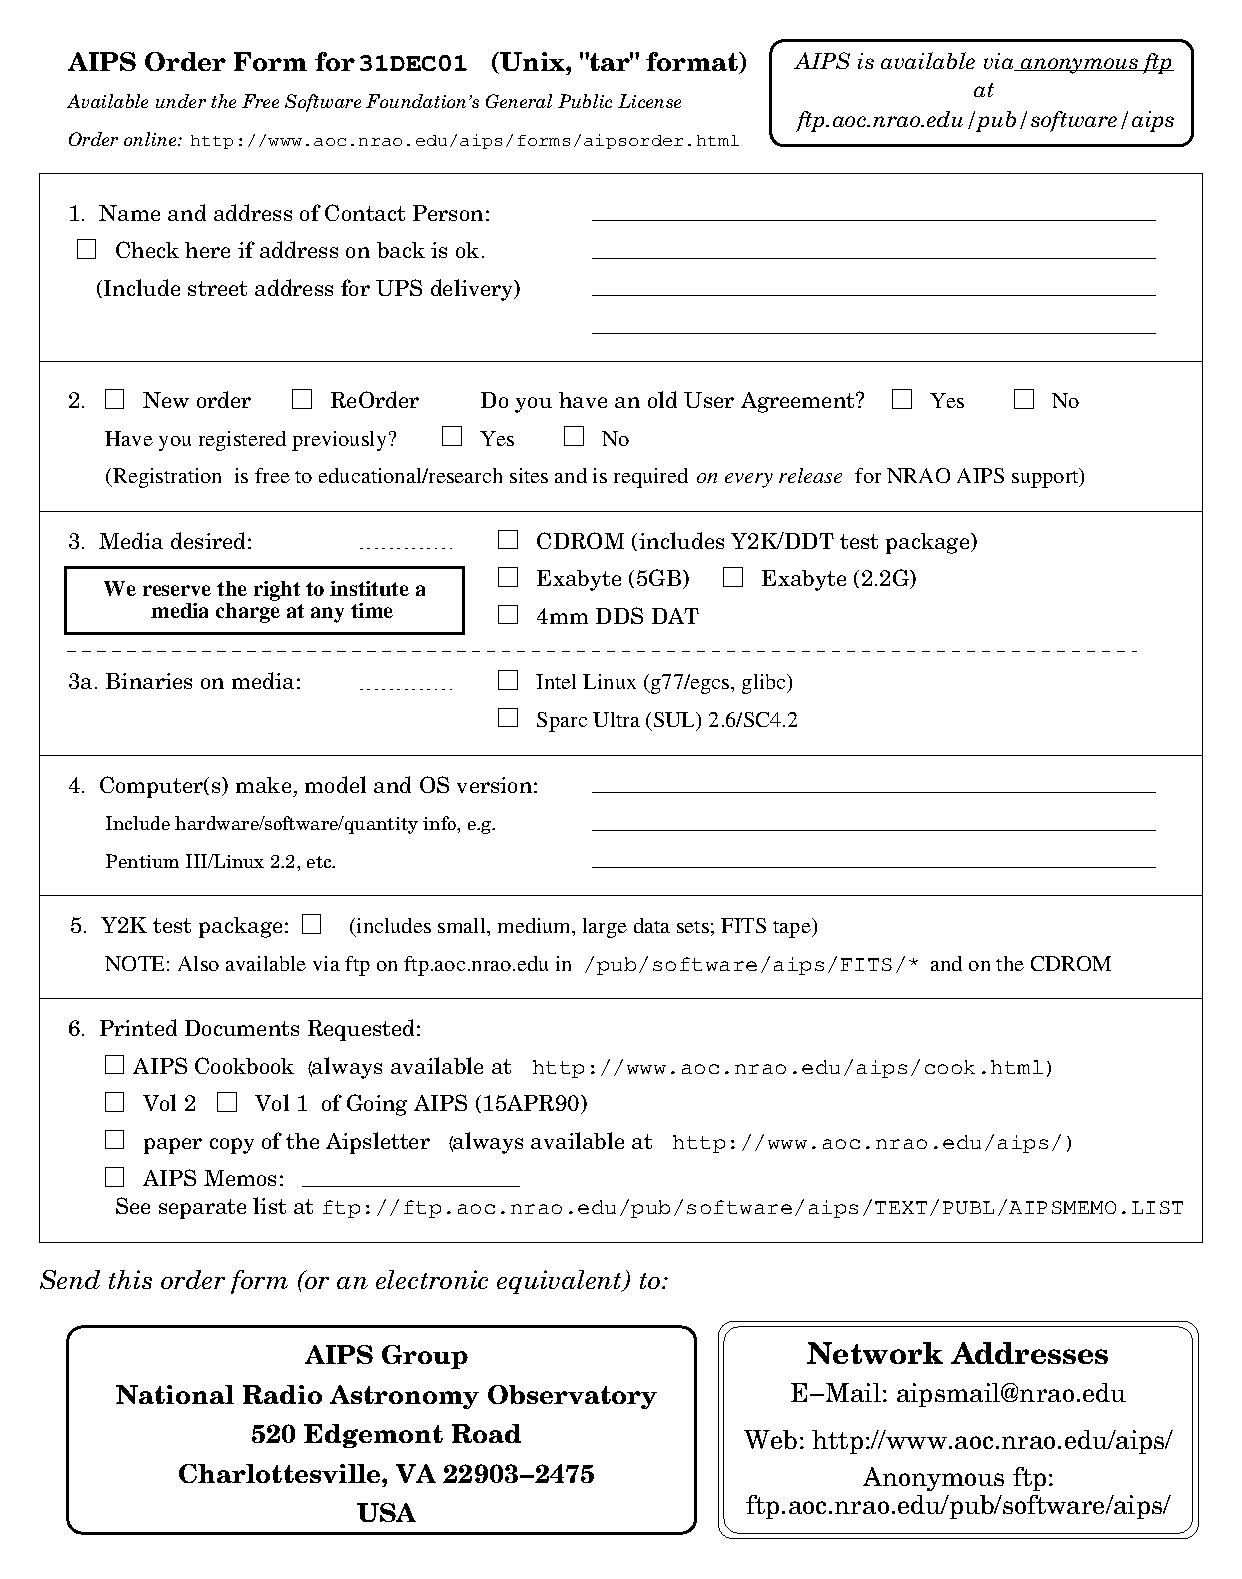
\includegraphics{FIG/AIPSORDER.PS}}}
%\vfill\eject
\vbox to 4.4in{
\vspace{12pt}
%\centerline{\rotatebox{-90}{\resizebox{!}{3.5in}{%
%\includegraphics{FIG/Mandrill.color.plt}}}}
\centerline{\resizebox{!}{3.5in}{\includegraphics{FIG/Mandrill.eps}}}
\vspace{12pt}
\centerline{{\huge \tt \AIPRELEASE}}
\vspace{12pt}
\vfill}
\phantom{...}
\centerline{\resizebox{!}{!}{\includegraphics{FIG/AIPSLETS.PS}}}

\end{document}
